\documentclass[10pt,letterpaper,twocolumn]{article}

\usepackage[top=2.1cm,left=2.0cm,right=2.0cm,footskip=2.0cm]{geometry}
\usepackage[utf8]{inputenc}     % for Unicode
\usepackage{cite}               % citation
\usepackage[dvipdfmx]{hyperref} % links
\usepackage{caption}            % caption
\usepackage{microtype}          % improves typesetting in LaTeX
\usepackage{algpseudocode}
\usepackage{algorithm}
\usepackage{graphicx}
\usepackage{color} % ex.) \textcolor{color}{text}

\renewcommand{\algorithmicrequire}{\textbf{Input:}}
\renewcommand{\algorithmicensure}{\textbf{Output:}}

\begin{document}

\twocolumn[
    \begin{flushleft}
        {\Large
        \textbf\newline{An Extention of R-Tree for Periodic Boundary Conditions}
        }
        \newline
        \\
        Toru Niina \textsuperscript{1}
        \\
        \bigskip
        \bf{1.} Department of Biophysics, Graduate School of Science,
                Kyoto University, Kyoto 606-8502, Japan
        \\
        \bigskip
        * niina@theory.biophys.kyoto-u.ac.jp
    \end{flushleft}

    \section*{Abstract}
    Searching spatial data is an important operation for scientific simulations
    which are performed mostly on periodic boundary conditions.
    An R-Tree is a widely used tree data structure to contain spatial objects and
    it is capable of answering to spatial searching queries in an efficient way.
    In this paper, I propose a novel method to construct R-Tree according to
    periodic boundary conditions by introducing a set of operations for
    rectangles.
    Unlike existing methods, this method works without any kind of additional
    copies of objects or queries.
    Moreover, because this method reduces the size of bounding boxes for each
    nodes of R-Tree in the natural way in the conditions, it is expected to
    increase the efficiency of processing spatial queries.
    The method can essentially be applied not only to the Guttman's original
    R-Tree but also to other data structures or algorithms if they use rectangles
    on periodic boudary conditions. The implementation is available on GitHub.
    \bigskip
]

\section*{Introduction}

Computational simulations are essential tools for scientific research, such as
investigating behaviors of complex biochemical models. To perform such a large
scale simulation, both huge amount of computational resources and efficient
simulation softwares are required.

In most cases, searching for objects that satisfy some geometrical conditions
is one of the most costly operation in the simulation. Generally, an efficient
method for spatial search drastically accelerates not only the whole simulation
processes, but also the data analysis of simulation results. Therefore, a method
that efficiently processes spatial search accelerates whole process of scientific
simulation research.

An R-Tree is a widely used data structure representing bounding volume
hierarchies (BVH) by using axis-aligned bounding box (AABB) for all its entries
\cite{Guttman1984}. It is capable of containing both sizeless and finite sized
objects such as points, segments, spheres and etc. As its efficiency, many
variants have been proposed and are applied for many problems in a broad range
of fields.

In order to use it with periodic boundary conditions (PBCs), currently,
two methods are proposed (figure\ref{fig-method-rtree-pbc})\cite{CoSTR-R-tree2016}.
The method that is visually described in figure \ref{fig-method-rtree-pbc}A
periodically copies all the objects in the simulation system along each dimension.
Although it can search objects associated with the adjacent periodic images in
the same way as normal R-Tree, it consumes memory $3^D$ fold a lot (here $D$
reprecents a number of dimension).
Figure \ref{fig-method-rtree-pbc}B showes another method copies not the whole
system but a query in the same manner if the query goes outside of the boundary.
Although it works completely fine with sizeless particles, it has a limitation on
containing finite-sized objects. It might overlook objects if query is not copied
when it is inside of the boundary and objects extend beyond the unit cell
(figure\ref{fig-method-rtree-pbc}C).

Here I propose the novel method to apply PBCs to an R-Tree. The main idea is
applying the PBCs to each operations for AABBs that are performed in each step
to maintain an R-Tree. By allowing an AABB corresponding to each node to extend
along PBCs, an R-Tree become capable of containing objects in the most natural
way on PBCs and overcoming the limitation of containing finite-sized object
(figure\ref{fig-method-rtree-pbc}CD).
With this method, it is not needed to copy objects or queries at all.
Moreover, using the information about the boundary condition, it has more chance
to reduce the AABBs of each node. Since the efficiency of spatial searching on
an R-Tree is strongly affected by the size of each nodes, this feature increase
the efficiency of spatial searching in some cases.

\begin{figure}[hbt]
    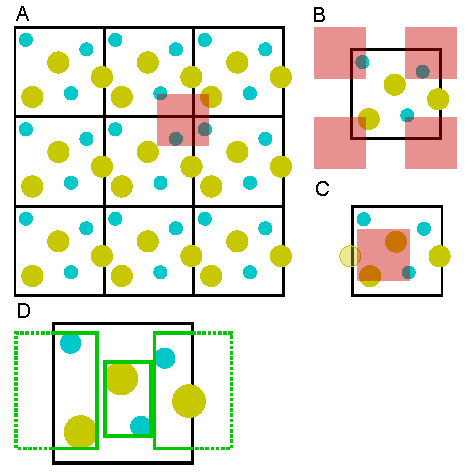
\includegraphics[width=8.4cm, bb=6 3 220 224]{fig1.eps}
    \caption{Methods to handle R-Tree on periodic boundary conditions.
    (\textbf{A})
    By copying the unit cell for each dimension along periodicity, normal R-Tree
    can manage objects that are associated with periodic images.
    (\textbf{B})
    By adding extensional query translated for each periodic images, R-Tree can
    detect objects that are beyond boundary.
    (\textbf{C})
    With the method described in \textbf{B}, finite sized objects could be
    overlooked when queries that is inside of the boundary are not copied.
    (\textbf{D})
    This is the method proposed in this paper. Forming rectangles according to
    the periodicity, R-Tree can organize objects on periodic boundary
    conditions.}
    \label{fig-method-rtree-pbc}
\end{figure}

\section*{Methods}

Here I introduce some operations to modify and handle rectangles on PBCs.
I do not modify the algorithm to grow and maintain an R-Tree at all.
Hence, in this setion, I do not show algorithm to construct R-Tree itself.
It means that this method can potentially be applied for some of the R-Tree
variants and the other spatial indexing methods that uses AABBs.

Because the rectangles that are used in R-Tree are axis-aligned, it is
enough to show the operation for one dimension to provide the whole algorithm.
Applying those procedure to each dimensions successively, these operations can
easily be extended for higher dimension cases.

\paragraph{Representation of the PBCs.}
As an unit cell of the PBCs, I consider only cuboids.
It make the rectangle operations on the condition drastically easier compared to
other shape of unit cells.
I restrict coordinates of all the objects to inside of the unit cell.
There are well-known alrogithm to restrict coordinates and vectors to the unit
cell. In this paper, I call them as \textbf{RestrictPosition} and
\textbf{RestrictVector}, respectively.

\paragraph{Representation of an rectangles.}
There are some options to represent an rectangle.
For example, a pair of coordinates describing upper and lower limit in each
dimensions is the widely used representation of an axis aligned rectangle.
Besides, a rectangle can be represented as a pair of coordinate and
vector describing its characteristic position such as centroid or lower limit
and width of rectangle in each dimension.
Because the method proposed in this paper quite often uses centroids of
rectangles, here I represent a rectangle as a pair of centroid position and
width vector.

\begin{equation}
    rectangle = \{centroid, width\}
\end{equation}

Of course, all the representations have identical information, one can easily
convert a certain representation to another. By algorithm\ref{centroid_aabb} and
\ref{width_aabb}, one can easily convert the upper-lower representation to
the centroid-width representation.

\begin{figure}[hbt]
    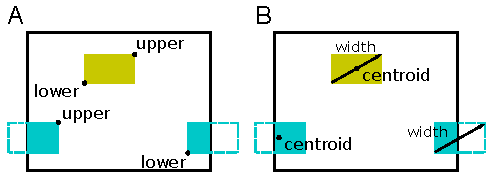
\includegraphics[width=8.4cm, bb=3 2 233 83]{fig3.eps}
    \caption{
    (\textbf{A})
    Representation of rectangle as a pair of upper and lower coordinates.
    (\textbf{B})
    Representation of rectangle as a pair of a centroid and width vector.
    }
    \label{fig-rectangle-rep}
\end{figure}

\begin{algorithm}
    \caption{calculate the centroid of an AABB on PBCs.}
    \label{centroid_aabb}
    \begin{algorithmic}
        \State $U \gets$ upper limit of AABB restricted in the unit cell
        \State $L \gets$ lower limit of AABB restricted in the unit cell
        \State $B \gets$ the unit cell of a boundary
        \Function{CentroidAABB}{$U, L, B$}
            \If{$U < L$}
                \State $C \gets (U + B.width + L) / 2$
            \Else
                \State $C \gets (U + L) / 2$
            \EndIf
            \State \Return $C$
        \EndFunction
     \end{algorithmic}
\end{algorithm}

\begin{algorithm}
    \caption{calculate the width of an AABB on PBCs.}
    \label{width_aabb}
    \begin{algorithmic}
        \State $U \gets$ upper limit of AABB restricted in the unit cell
        \State $L \gets$ lower limit of AABB restricted in the unit cell
        \State $B \gets$ the unit cell of a boundary
        \Function{WidthAABB}{$U, L, B$}
            \If{$U < L$}
                \State $W \gets U + B.width - L$
            \Else
                \State $W \gets U - L$
            \EndIf
            \State \Return $W$
        \EndFunction
     \end{algorithmic}
\end{algorithm}

\paragraph{Expanding AABBs on PBCs.}
Expanding an AABB to make it a minimal bounding box of its contents is one of
the most important operations done to form R-Tree.
Because the total area that is covered by AABBs in the nodes of R-Tree affects
the efficiency of spatial searching, it is needed to find the way to make the
area of rectangle in each node as small as possible.

The algorithm to find the minimum expansion of AABB to contain another AABB on
PBCs is shown in algorithm ~\ref{expand_aabb_aabb}.
The size of bounding box that contains two rectangles is determined by the
distance between their centroids because of the symmetry of a rectangule.
Therefore, by minimizing the distance between their centroids, the minimum
expansion can be found. To minimize the distance between two points on PBCs,
the \textbf{RestrictVector} can be used.

\begin{algorithm}
    \caption{expand AABB so that it contains another AABB}
    \label{expand_aabb_aabb}
    \begin{algorithmic}
        \State $R1 \gets$ AABB to be expanded
        \State $R2 \gets$ rectangle to be contained
        \State $B  \gets$ boundary
        \Function{ExpandAABB}{$R1, R2, B$}
            \State $dc \gets R2.centroid - R1.centroid$
            \State $dc \gets$ \Call{RestrictVector}{dc, B}

            \State $l1 \gets R1.centroid - R1.width / 2$
            \State $u1 \gets R1.centroid + R1.width / 2$
            \State $l2 \gets (R1.centroid + dc) - R2.width / 2$
            \State $u2 \gets (R1.centroid + dc) + R2.width / 2$

            \State $L \gets \Call{min}{l1, l2}$
            \State $U \gets \Call{max}{u1, u2}$
            \State $C \gets (L + U) / 2$
            \State $W \gets U - L$
            \State $C \gets$ \Call{RestrictPosition}{C, B}

            \State \Return $\{C, W\}$
        \EndFunction
     \end{algorithmic}
\end{algorithm}

For the case of containing points, it become simpler as described in the
algorithm ~\ref{expand_aabb_point}. By minimizing the distance between centroid
of the rectangle and the point to be contained, the minimum expansion can be
implemented.

\begin{algorithm}
    \caption{expand AABB so that it contains a point}
    \label{expand_aabb_point}
    \begin{algorithmic}
        \State $R \gets$ AABB to be expanded
        \State $P \gets$ point to be contained
        \State $B \gets$ boundary
        \Function{ExpandAABB}{$R, P, B$}
            \State $dc \gets P - R.centroid$
            \State $dc \gets$ \Call{RestrictVector}{dc, B}

            \State $l \gets R.centroid - R.width / 2$
            \State $u \gets R.centroid + R.width / 2$

            \State $L \gets \Call{min}{l, P}$
            \State $U \gets \Call{max}{u, P}$
            \State $C \gets (L + U) / 2$
            \State $W \gets U - L$

            \State $C \gets$ \Call{RestrictPosition}{C, B}
            \State \Return $\{C, W\}$
        \EndFunction
     \end{algorithmic}
\end{algorithm}

\paragraph{Detecting an object includes or intersects the other object}

To find an object in an R-Tree, it is needed that the way to check whether an
rectangle intersects or be inside of an rectangle.
It also can be determined by using the minimum distance between centroids of the
rectangles.
Figure ~\ref{fig-geometric-relationship} graphically shows the idea of each
algorithms in 1 dimension.

\begin{algorithm}
    \caption{Check whether an AABB is inside of an AABB}
    \begin{algorithmic}
        \State $R1 \gets$ rectangle
        \State $R2 \gets$ rectangle that might be inside of R1
        \State $B  \gets$ boundary
        \Function{IsAABBInsideOfAABB}{$R1, R2, B$}
            \State $dc \gets R1.centroid - R2.centroid$
            \State $dc \gets$ \Call{RestrictVector}{dc, B}

            \State \Return \Call{abs}{dc} $\leq (R1.width - R2.width) / 2$
        \EndFunction
     \end{algorithmic}
\end{algorithm}

\begin{algorithm}
    \caption{Check whether a point is inside of an AABB}
    \begin{algorithmic}
        \State $R \gets$ rectangle
        \State $P \gets$ point that might be inside of R
        \State $B \gets$ boundary
        \Function{IsPointInsideOfAABB}{$R, P, B$}
            \State $dc \gets R.centroid - P$
            \State $dc \gets$ \Call{RestrictVector}{dc, B}
            \State \Return \Call{abs}{dc} $\leq (R.width) / 2$
        \EndFunction
     \end{algorithmic}
\end{algorithm}

\begin{algorithm}
    \caption{Check whether an AABB intersects to another AABB}
    \begin{algorithmic}
        \State $R1 \gets$ rectangle
        \State $R2 \gets$ rectangle that might intersect to R1
        \State $B  \gets$ boundary
        \Function{IntersectsAABB}{$R1, R2, B$}
            \State $dc \gets R.centroid - R.centroid$
            \State $dc \gets$ \Call{RestrictVector}{dc, B}
            \State \Return \Call{abs}{dc} $\leq (R1.width + R2.width) / 2$
        \EndFunction
     \end{algorithmic}
\end{algorithm}

\begin{figure}[thb]
    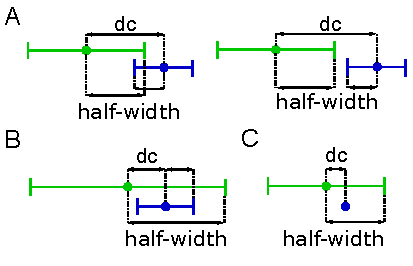
\includegraphics[width=8.4cm, bb=1 9 196 125]{fig2.eps}
    \caption{
    Visual description of geometrical relationships.
    (\textbf{A})
    Intersection detection of rectangles by widths and centroids. If sum of half
    width is less than the distance between centroids, the rectangles intersect.
    (\textbf{B})
    Inclusion detection of rectangles. If sum of distance between centroids and
    half width of the rectangle that might be included is less than the half
    width of the rectangle that might includes the other, the rectangles have
    including-included relationship.
    (\textbf{C})
    For point, intersection and inclusion means the same thing. If the distance
    between the centroid of the rectangle and the point is less than the half
    width of the centroid, the point intersects to the rectangle.
    }
    \label{fig-geometric-relationship}
\end{figure}

\section*{Conclusion}

In this paper, the novel method for applying PBCs to Guttman's R-Tree is
introduced. Proposed method is capable of containing not only sizeless points
but also objects with finite size. The method can remove the necessity of
storing extensional objects or replicating queries. Moreover, it reduces the
size of each node in the natural way on PBCs.

On the other hand, the method introduces tiny but additional costs into each
procedures for maintaining R-Tree and checking geometrical conditions because it
considers the PBCs for all of the procedure. It might decrease the efficiency of
the R-Tree in some case.

As described before, since the method is only for modifying and handling
rectangles on PBCs, it can essentially be applied for the other R-Tree variants
or the other kind of spatial indexing methods.

Because the adaptation of spatial indexing to a system on PBCs has a chance to
accelerate many kind of sientific simulations, it is expected that this novel
method will have an important role for the simulations that will be performed in
the next decade.

\bibliographystyle{plain}
\bibliography{library}{}

\end{document}
